\documentclass[12pt]{beamer}
\usetheme{CambridgeUS}
\usepackage[utf8]{inputenc}
\usepackage[spanish]{babel}
\usepackage{amsmath}
\usepackage{amsfonts}
\usepackage{amssymb}
\usepackage{graphicx}
\author{Kevin Garcia - Cesar Saavedra}
\title{Taller: Modelos de distribución}
%\setbeamercovered{transparent} 
%\setbeamertemplate{navigation symbols}{} 
%\logo{} 
%\institute{} 
%\date{} 
%\subject{} 
\begin{document}

\begin{frame}
\titlepage
\end{frame}

%\begin{frame}
%\tableofcontents
%\end{frame}
\begin{frame}
\frametitle{Distribución Poisson}
~\\  Esta distribución es una de las más importantes distribuciones de variable discreta. Sus principales aplicaciones hacen referencia a la modelización de situaciones en las que nos interesa determinar el número de hechos de cierto tipo que se pueden producir en un intervalo de tiempo o de espacio, bajo presupuestos de aleatoriedad.
~\\ Su función de densidad esta dada por: 
~\\$$f(x,\lambda)=\frac{e^{-\lambda}\cdot \lambda^x}{x!}  ; x \in \{0,1,2,3,...\}$$
~\\donde:
\begin{itemize} 
\item x es el número de ocurrencias del evento o fenómeno (la función nos da la probabilidad de que el evento suceda precisamente x veces).
\end{itemize}
\end{frame}

\begin{frame}
\frametitle{Distribución Poisson}
\begin{itemize}
\item $\lambda$ es un parámetro positivo que representa el número de veces que se espera que ocurra el fenómeno durante un intervalo dado.
\item $F(x)=\sum\limits_{i=1}^{x} \frac{\lambda_{i}\cdot e^{-\lambda}}{i!}=\frac{\Gamma([k+1],\lambda)}{[k]!}$ para $k>0$ y $\Gamma(x,y)$ es la función gamma incompleta.
\item $f.g.m=m_{x}(t)=E[e^{tx}]=\sum\limits_{x} e^{tx}p(x)= e^{[\lambda(e^t-1)]}$
\item $Media=E[x]=\lambda$
\item $Varianza=\lambda$
\item Coeficiente de asimetría=$\frac{1}{\sqrt{\lambda}}$
\item curtosis=$3+\frac{1}{\lambda}$
\end{itemize}
\end{frame}

\begin{frame}
\frametitle{Aplicaciones de la distribución Poisson}
~\\La distribución de Poisson se emplea para describir procesos como los siguientes:  
\begin{itemize}
\item El número de autos que pasan a través de un cierto punto en una ruta (suficientemente
distantes de los semáforos) durante un periodo definido de tiempo.  
\item El número de errores de ortografía que uno comete al escribir una única página.  
\item El número de llamadas telefónicas en una central telefónica por minuto.  
\item El número de servidores web accedidos por minuto.  
\item El número de defectos en una longitud específica de una cinta magnética.   
\item El número de defectos por metro cuadrado de tela.
\item El número de estrellas en un determinado volumen de espacio.
\end{itemize}
\end{frame}
\begin{frame}
\frametitle{Distribución Logística}
~\\La función de distribución de la logística es una distribución de probabilidad continua que se usa como modelo de crecimiento. Por ejemplo,
con un nuevo producto, a menudo encontramos que el crecimiento es inicialmente lento, luego gana impulso,
y finalmente se ralentiza cuando el mercado está saturado o hay alguna forma de equilibrio
alcanzado
~\\ Su función de densidad está dada por:
$$f(x;a,b)=\frac{e^{-(x-a)/b}}{b(1+e^{-(x-a)/b})^2}=\frac{1}{4b}sech^2\left(\frac{x-a}{2b}\right)$$
\end{frame}

\begin{frame}
\frametitle{Distribución Logística}
~\\ Su función de distribución está dada por:
$$F(x;a,b)=\frac{1}{1+e^{-(x-a)/b}}=\frac{1}{2}+\frac{1}{2}tanh\left(\frac{x-a}{2b}\right)$$
\begin{itemize}
\item $f.g.m=e^{at}\Gamma(1-bt)\Gamma(1+bt)=\pi bt\frac{e^{at}}{sin(\pi bt)}$
\item $Media=E[x]=a$
\item $Mediana=a$
\item $Moda=a$
\item $Varianza=\frac{\pi^2 b^2}{3}$
\end{itemize}
\end{frame}

\begin{frame}
\frametitle{Aplicaciones de la distribución Logística}
~\\ La distribución logística ha sido muy utilizada en áreas como:
\begin{itemize}
\item Biología: para describir cómo se comportan las especies en entornos competitivos.
\item Epidemiología: para describir la propagación de epidemias.
\item Psicología: para describir el proceso de aprendizaje.
\item Tecnología: para describir cómo las tecnologías se popularizan y compiten entre sí.
\item Márketing: para estudiar la difusión de nuevos productos.
\item Energía: para estudiar la difusión y sustitución de unas fuentes de energía primarias por otras.
\end{itemize}
\end{frame}

\begin{frame}
\frametitle{Comportamiento distribución Poisson}
\begin{figure}[!h]
    \begin{center}
        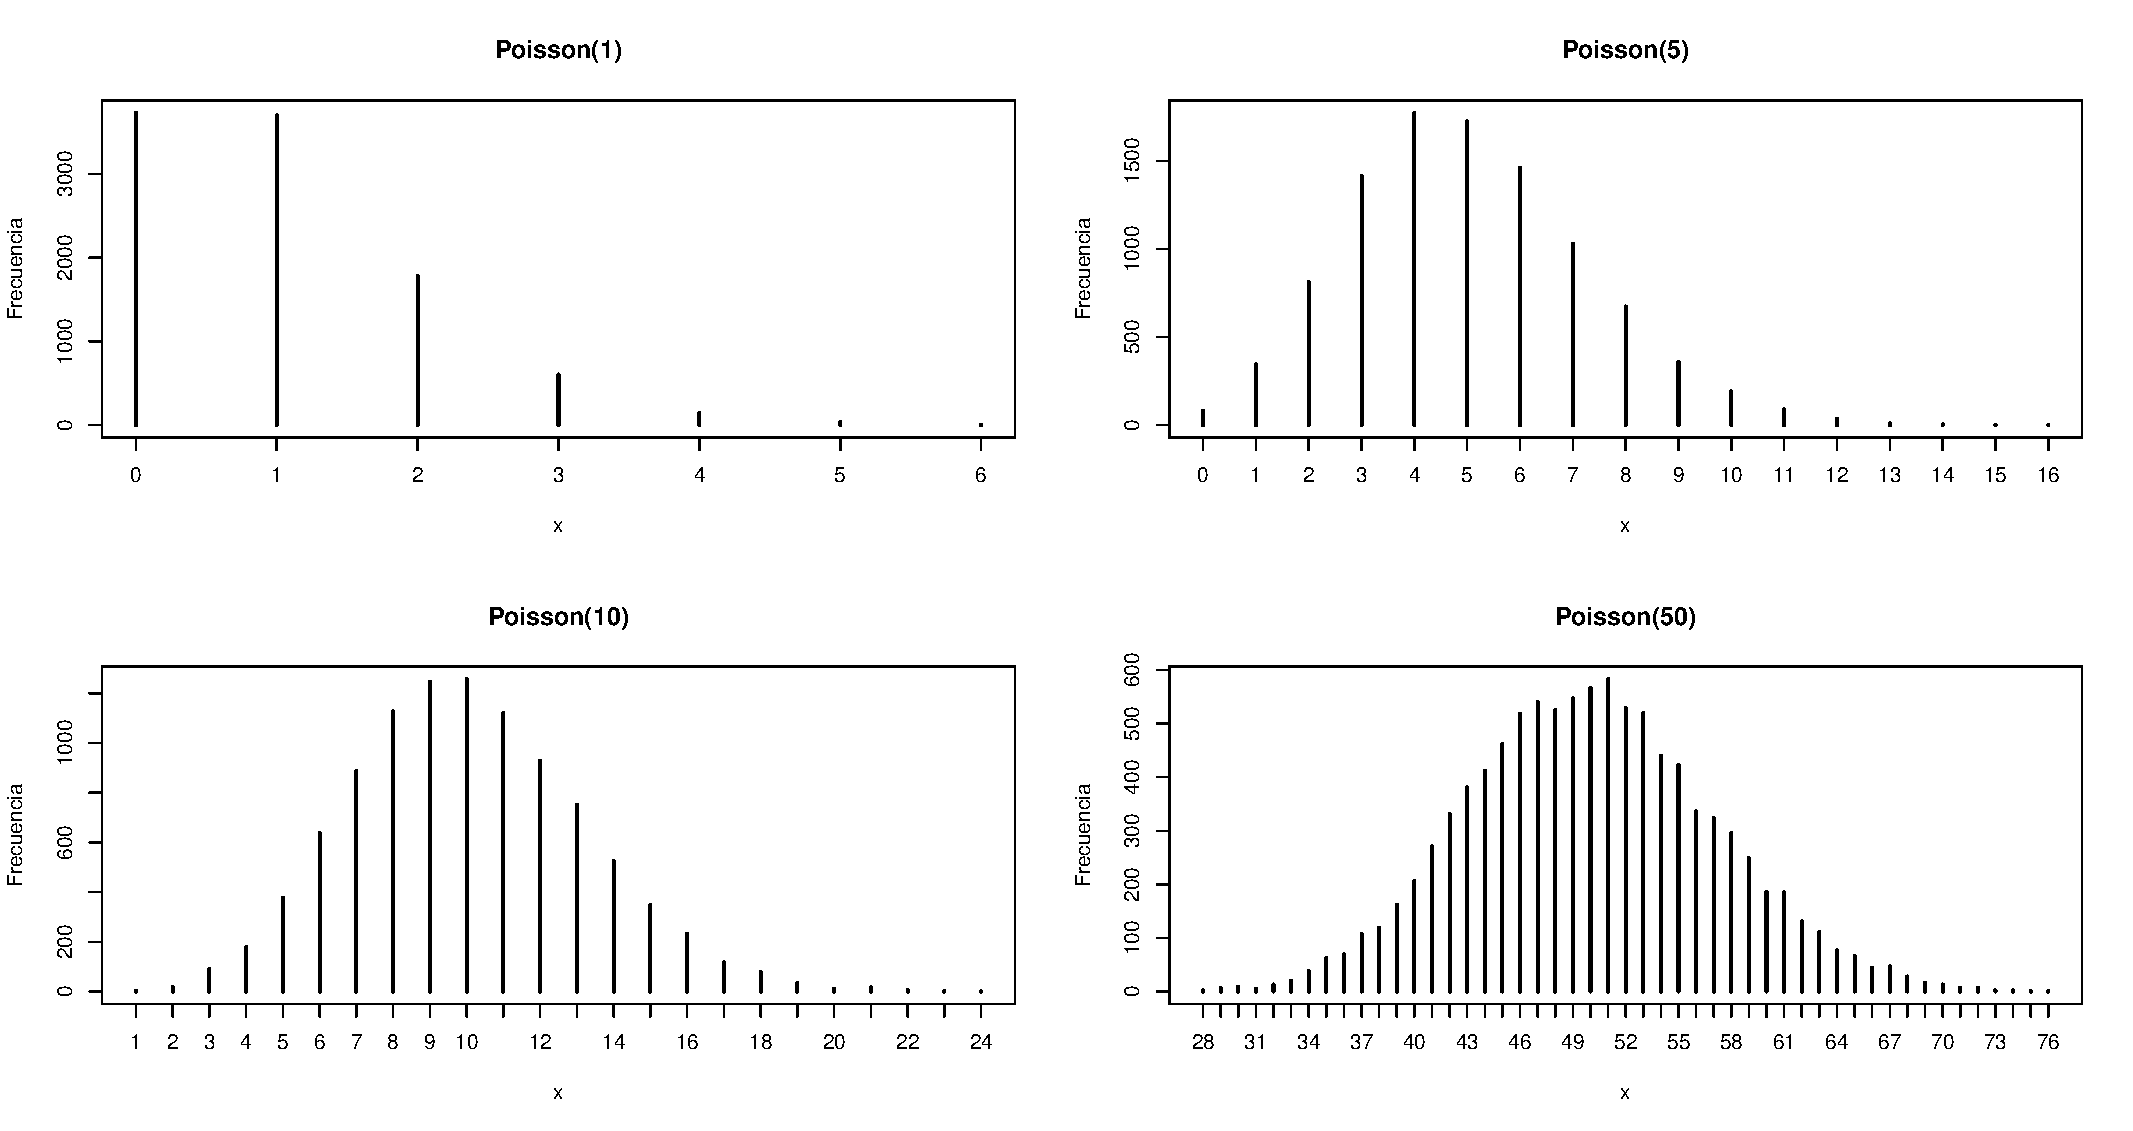
\includegraphics[width=11cm]{imagenes/poisson1.pdf}
        \caption{Comportamiento de la distribución Poisson variando $\lambda$}
        \label{fig:Densidad}
    \end{center}
\end{figure}
\end{frame}

\begin{frame}
\frametitle{Comportamiento distribución Logística}
\begin{figure}[!h]
    \begin{center}
        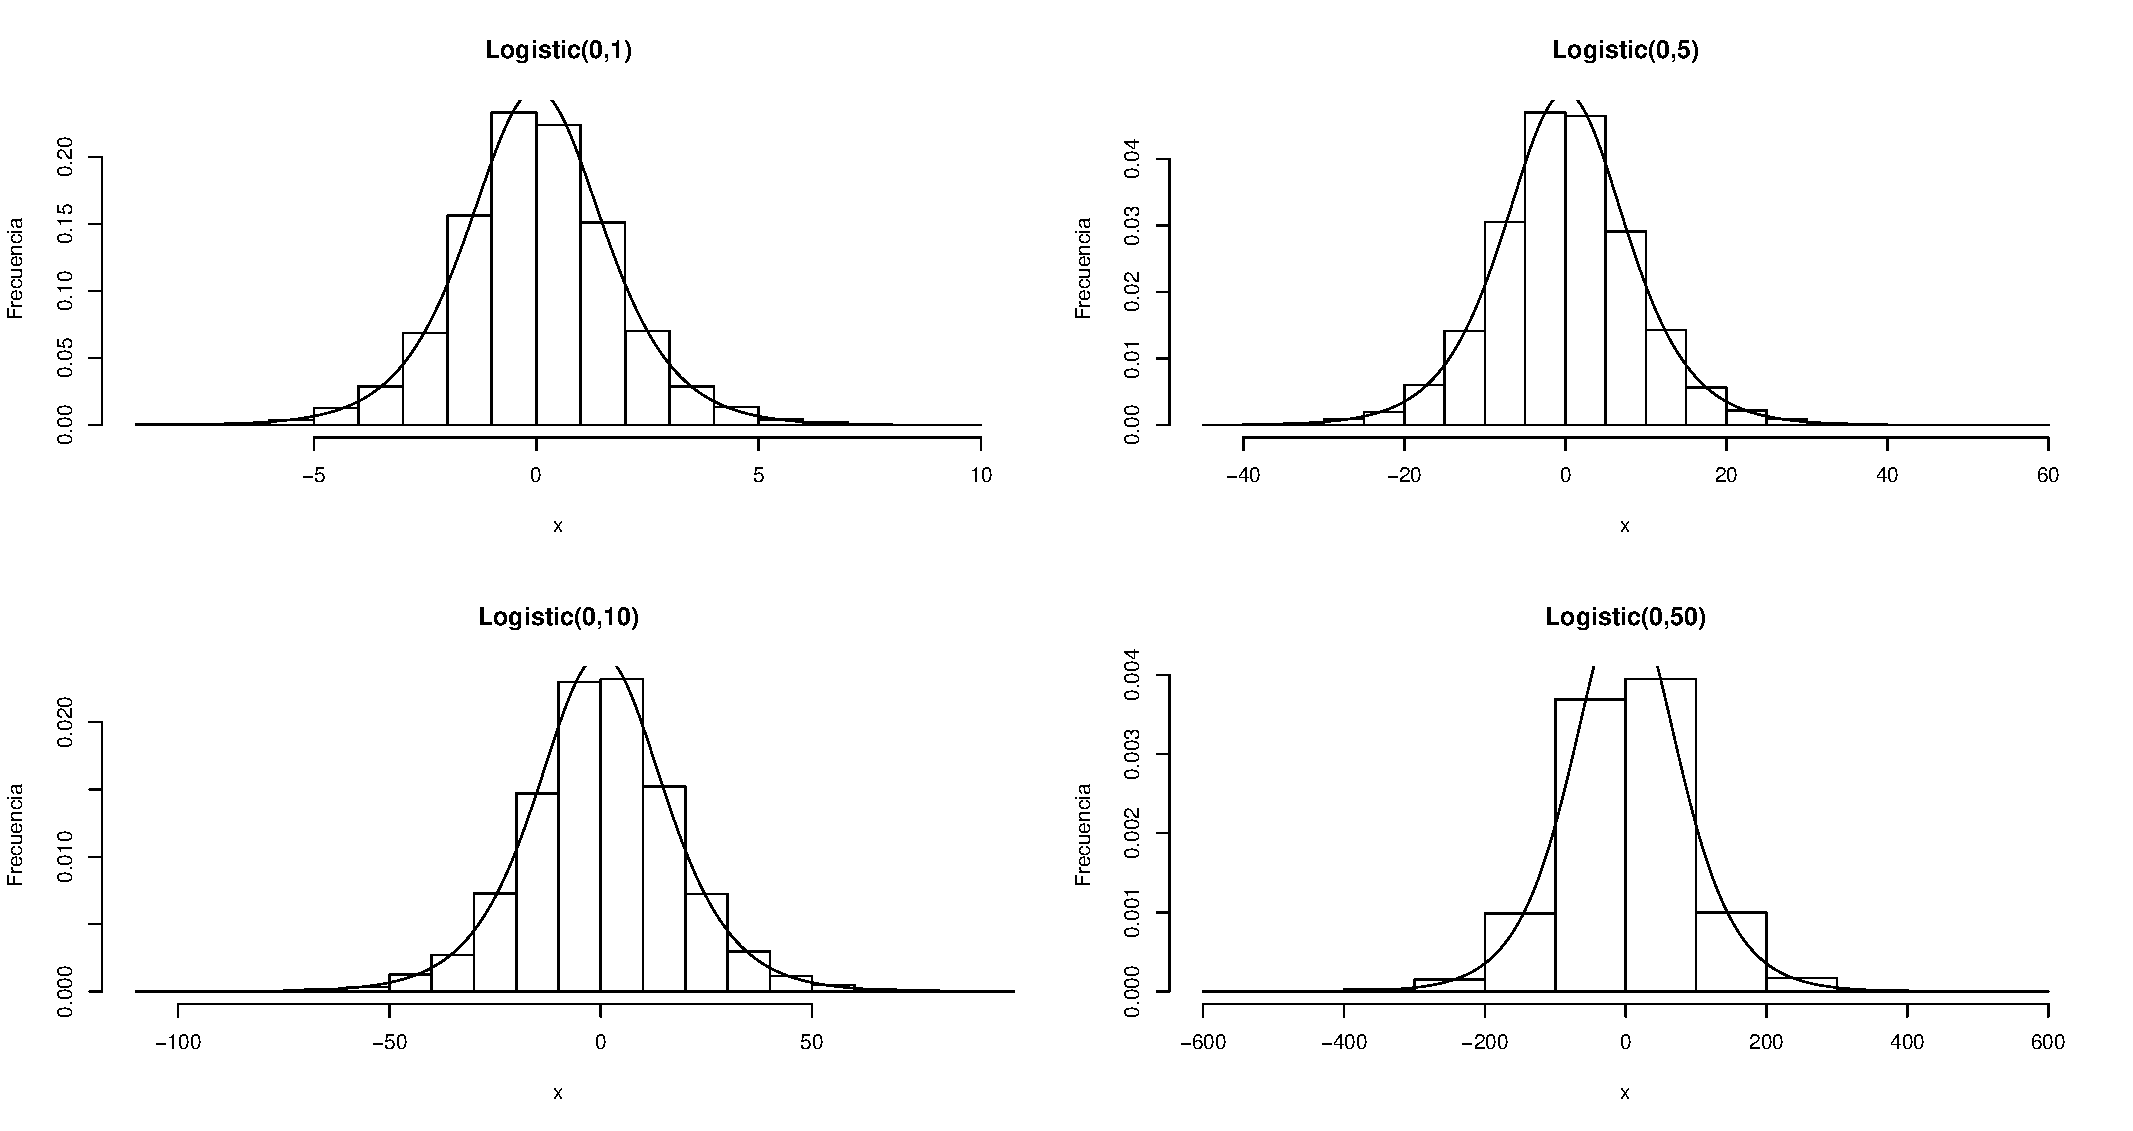
\includegraphics[width=11cm]{imagenes/logistic0.pdf}
        \caption{Comportamiento fijando localización y variando escala}
        \label{fig:Densidad}
    \end{center}
\end{figure}
\end{frame}

\begin{frame}
\frametitle{Comportamiento distribución Logística}
\begin{figure}[!h]
    \begin{center}
        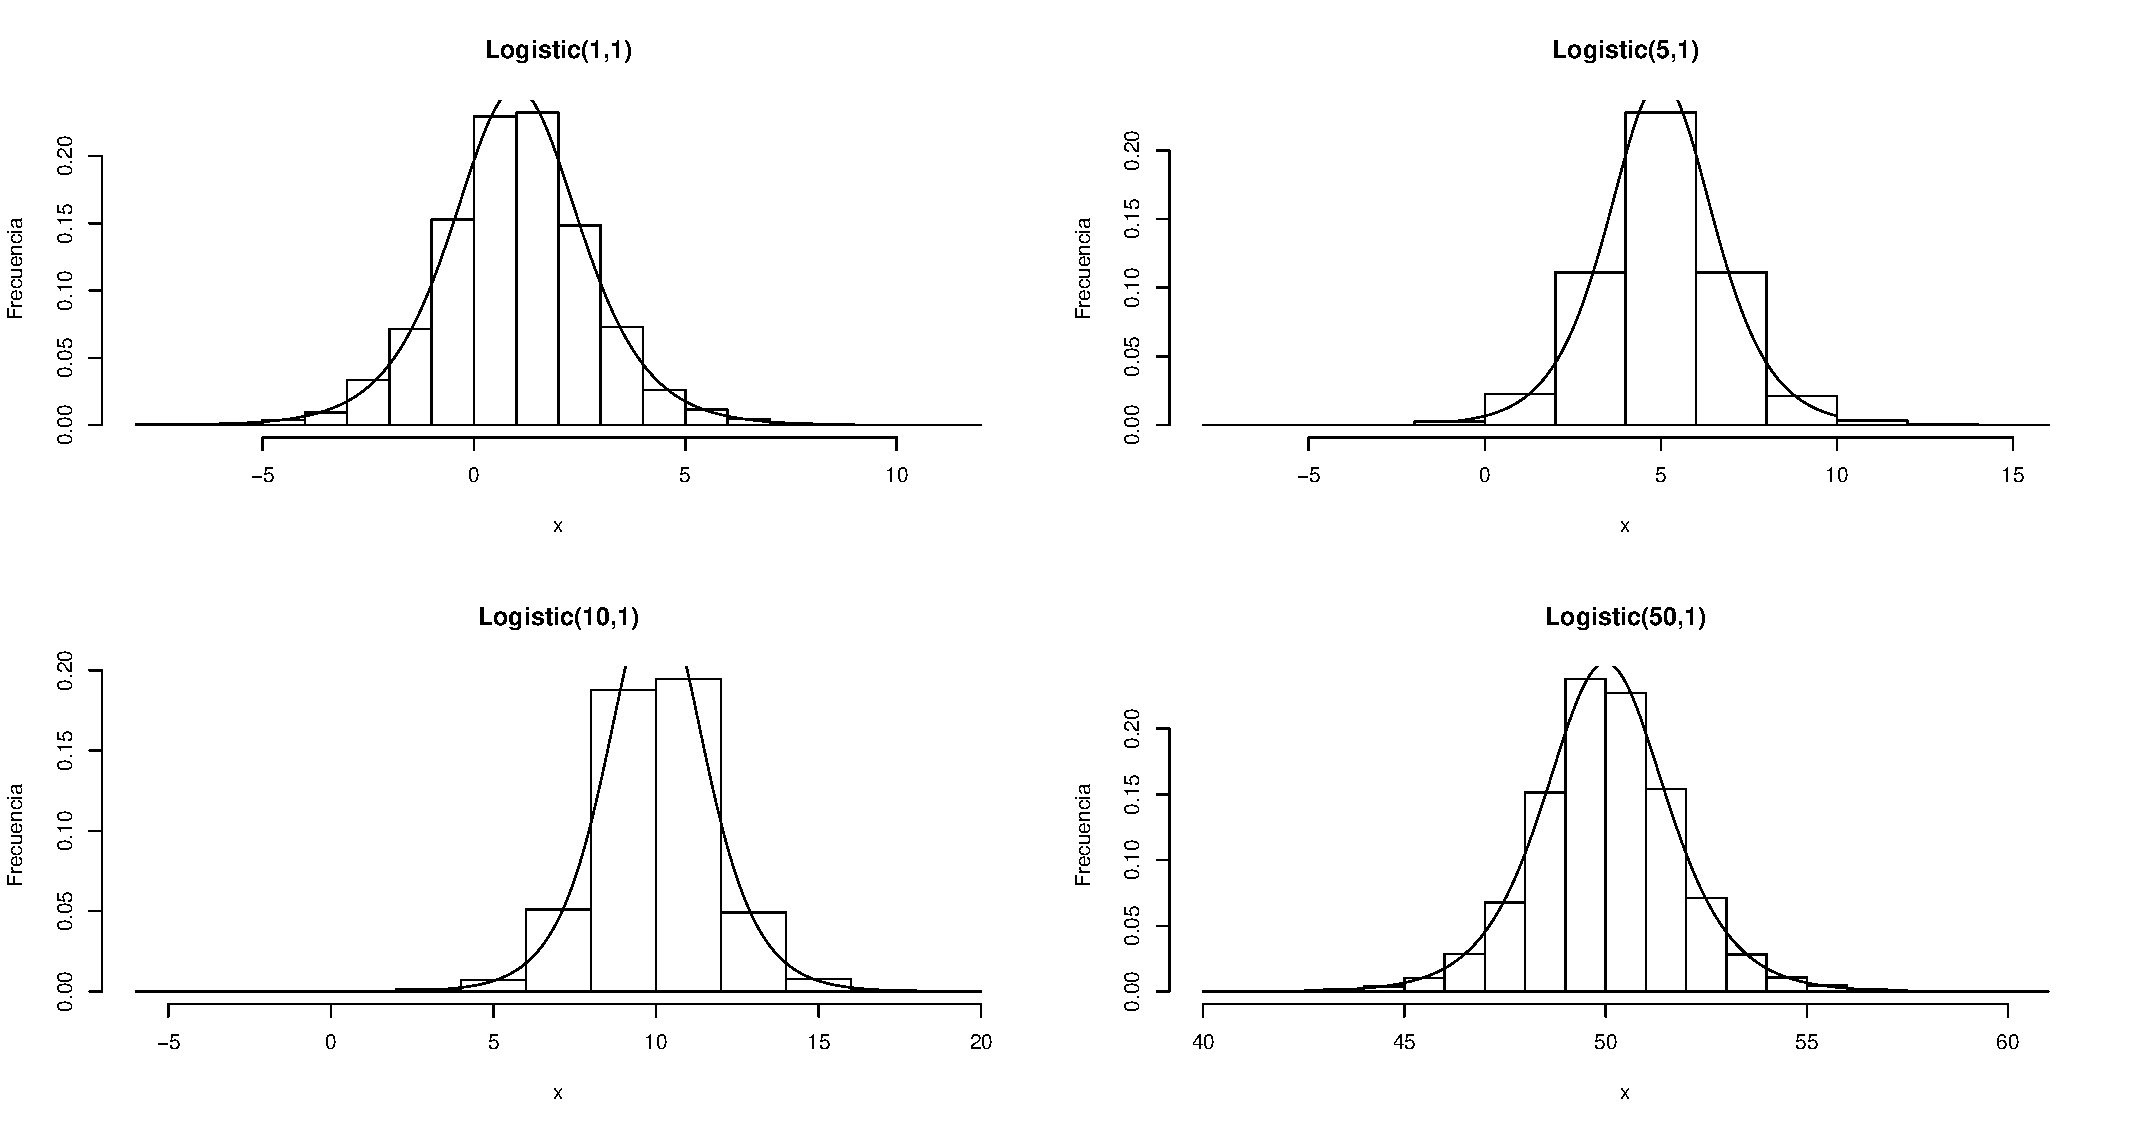
\includegraphics[width=11cm]{imagenes/logistic1.pdf}
        \caption{Comportamiento fijando escala y variando localización}
        \label{fig:Densidad}
    \end{center}
\end{figure}
\end{frame}

\end{document}